\chapter{Recursion}

Recursive functions are those which call themselves, for example, this implementation of the factorial function.

It might be difficult to understand at first, but it simplifies code once you get used to it. The best way to master it is through looking at more examples. You can see more examples on recursion in the mycodeschool playlist.

\section{Further resources: mycodeschool}

Playlists by 
\href{https://www.youtube.com/user/mycodeschool}{mycodeschool}\footnote{Link: \href{https://www.youtube.com/user/mycodeschool}{https://www.youtube.com/user/mycodeschool}}
that focuses on 
\href{https://www.youtube.com/watch?v=_OmRGjbyzno&list=PL2_aWCzGMAwLz3g66WrxFGSXvSsvyfzCO}{recursion}\footnote{Link: \href{https://www.youtube.com/watch?v=_OmRGjbyzno&list=PL2_aWCzGMAwLz3g66WrxFGSXvSsvyfzCO}{https://www.youtube.com/\\watch?v=\_OmRGjbyzno\&list=PL2\_aWCzGMAwLz3g66WrxFGSXvSsvyfzCO}}, 
\href{https://youtube.com/playlist?list=PL2_aWCzGMAwLZp6LMUKI3cc7pgGsasm2_}{pointers}\footnote{Link: \href{https://youtube.com/playlist?list=PL2_aWCzGMAwLZp6LMUKI3cc7pgGsasm2_}{https://youtube.com/playlist?list=PL2\_aWCzGMAwLZp6LMUKI3cc7pgGsasm2\_}} and 
\href{https://www.youtube.com/playlist?list=PL2_aWCzGMAwI3W_JlcBbtYTwiQSsOTa6P}{data structures (linked lists, stacks, queues)}\footnote{Link: \href{https://www.youtube.com/playlist?list=PL2_aWCzGMAwI3W_JlcBbtYTwiQSsOTa6P}{https://www.youtube.com/playlist?list=PL2\_aWCzGMAwI3W\_JlcBbtYTwiQSsOTa6P}}.
mycodeschool explains concepts about computing pretty well. You can watch his other playlists if interested.

\section{Example: Factorial function}

\begin{lstlisting}
int fact(int x){
    if(x==0) return 0;
    else return x*fact(x-1);
}
//What would happen if we input a negative number?
\end{lstlisting}

Internally, there is a \textbf{call stack}\index{call stack} to store information about each function call (e.g. the values of the variables, what is left to do) so that they could resume in order.

The figure shows what happens when I call fact(4)

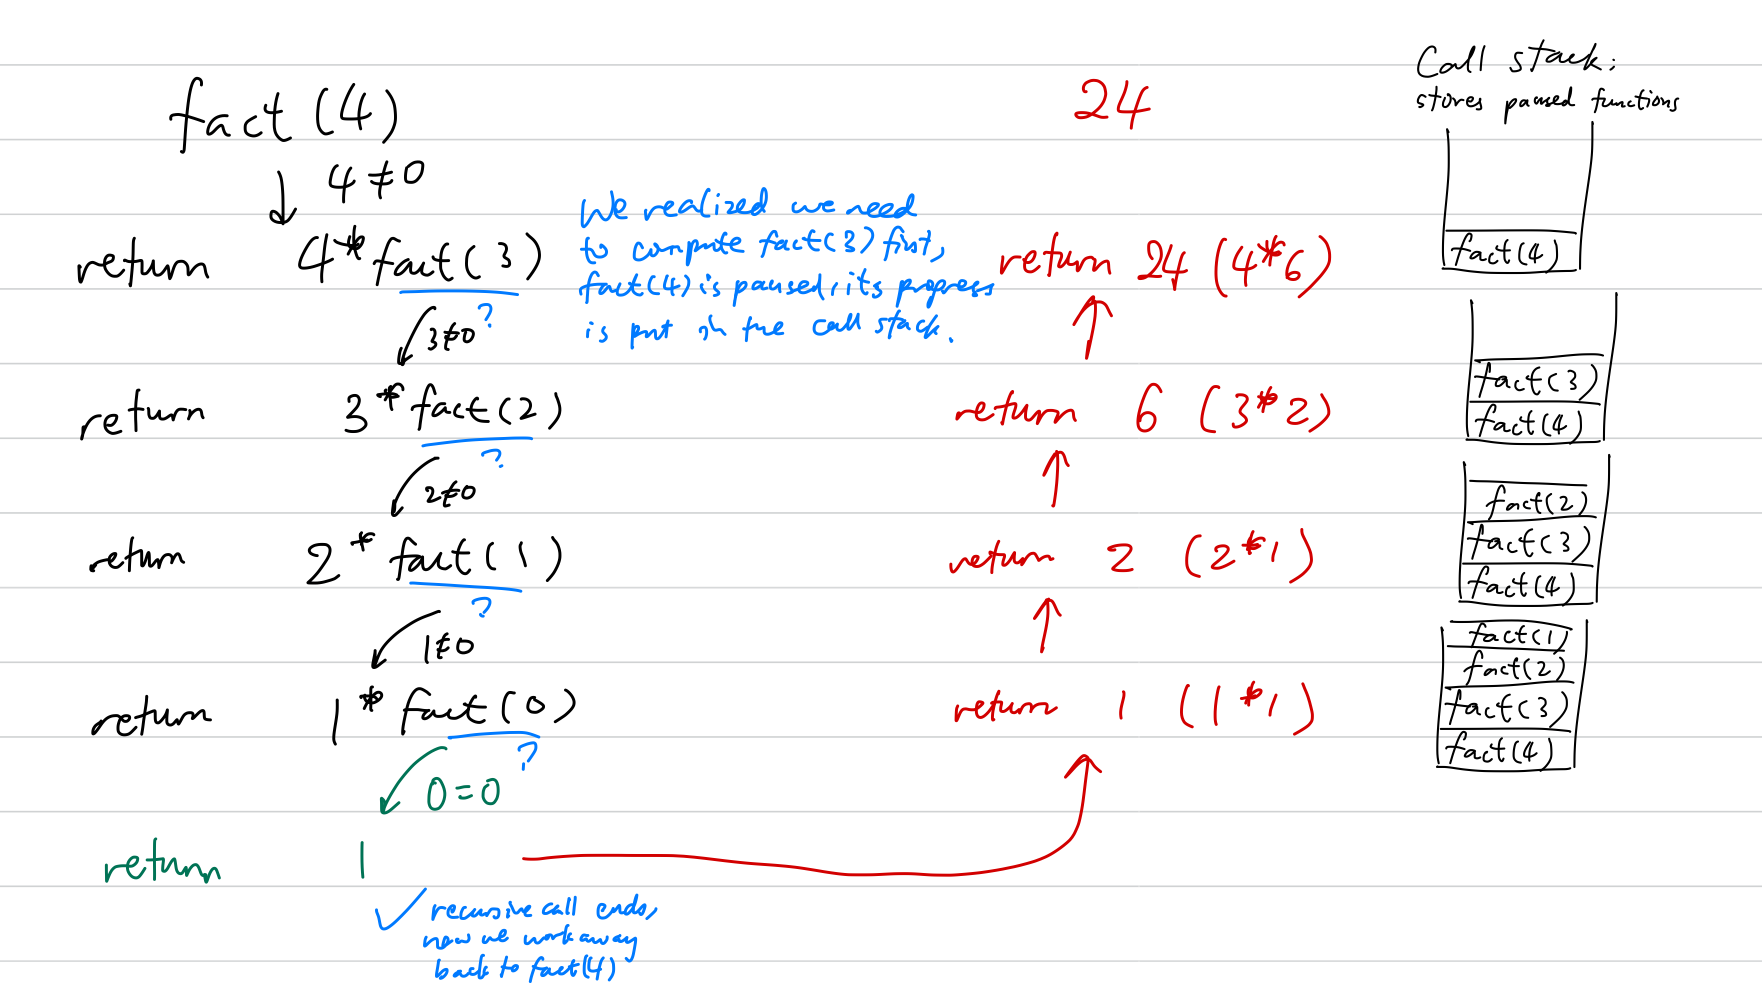
\includegraphics[width=15cm]{ch4-factorial.png}


